\chapter{Downwash Estimation}
\label{ch:workobject}
\markboth{Downwash Estimation}{}

\begin{flushright}
	{\smaller
		\textit{The important thing is not to stop questioning.\\  Curiosity has its own reason for existing.}\\
		-- Albert Einstein}
\end{flushright}

In order to evaluate the characteristics of longitudinal stability of an aircraft it's necessary to assess the flow direction aft of the wing. The contribution of horizontal tail surface to the airplane equilibrium and stability, in fact, depends seriously on the flow direction. The pourpose of this chapter is to introduce and evaluate the downwash gradient due from the wing's vortex system, considering a dependence of the downwash angle from the absolute angle of attack. 

\section{Theoretical background}

Due to the finite extension of the wing the lift distribution in span is not uniform. For this reason the difference of pressure between upper and lower surfaces generates a movement of air aroud the wingtips. The tendency is for particles of air to move from the region of high pressure around the wing tip to the region of low pressure (for positive lift from the lower wing surface to the upper surface). This made the wing's vortex system that consisting of the bound vortex, located at the wing quarter chord and a vortex sheet which rolling up, at the wing tip, in two trailing vortex.\cite{PerkinsHage} \cite{Jacobs:NACA:Rep:648} \\ 

% traduci

\begin{figure}[H]
\centering
{\includegraphics[height=5.7cm]{Immagini/wing_vortex_sheet3.pdf}} 
\caption{The wing vortex sheet.}
\end{figure}

The main effect of this vortex system is to deflect the airflow behind the wing downward relative to the direction of freestream flow. This angle of deviation is known as {\itshape Downwash Angle} $\epsilon$. This phenomenon occurs for every lifting surface, but in subsonic flow a lifting surface also affects the flow forward of itself. In this region the vortex creates an {itshape upwash}, that is an upward flow deflection.\\


\begin{figure}[H]
\centering
{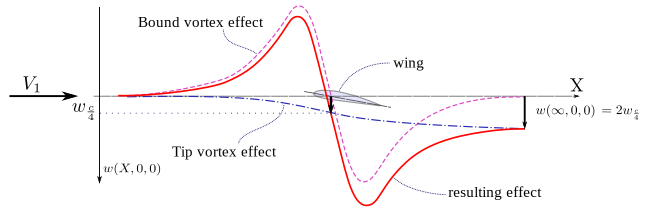
\includegraphics[height=5.16cm]{Immagini/wing_upwash_downwash.pdf}} 
\caption{Upwash and Downwash in a finite wing.}
\end{figure}

As consequence of the downwash behind the wing, the local angle of attack on the horizontal tail is reduced by  $\epsilon$. In order to evaluate the flow direction behind the wing, an other important parameter is the change in downwash angle with angle of attack, that is the {\itshape Downwash Gradient } $\frac{d\epsilon}{d\alpha}$.\\
This parameter depends principally on the location of the horizontal tail with respect to the wing and the vortex plane. As first approximation this value could be considered constant in alpha, but more accurately it's possible to evaluate this dependence considering the reference variable for the calculation of the distances. 
Both if the vertical distance is considered as constant and it is considered variable with alpha, starting from the downwash gradient, the downwash angle is :

\begin{equation}
\epsilon = \frac {d \epsilon}{d \alpha_w} (\alpha_w - \alpha_{0_w})
\end{equation}

\noindent \\ \\
In order to evaluate the downwash gradient it refers to fig. \ref{PerkinsDownwash}, where ``$r \frac{b}{2}$''  is the distance between the aerodynamic center of wing and the aerodynamic center of the horizontal tail. This is a geometric an fixed distance. Conversely, in order to have a greater accuracy it's possible to consider the distance ``$m  \frac{b}{2}$'' variable with the angle of attack. Properly this is the distance between the horizontal tail and the vortex shed plane, but it's possible to approximate it with the distance between the horizontal tail and the wing root chord.\cite{schimidth}

Referring to % fonte formula 
the equation used in order to evaluate the downwash gradient is the following: 

\begin{equation}
\begin{split}
 \frac{d\epsilon}{d\alpha} &= \frac{K_{\epsilon \Lambda}}{K_{\epsilon _{\Lambda=0}}}  \Biggr ( \frac{r}{r^2+m_{tv}^2} 
 \frac{0.4876}{\sqrt{r^2 + 0.6319 + m_{tv}^2}}  +\\
& \left [1+{ \left( \frac{r^2}{r^2 + 0.7915 + 5.0734 m_{tv}^2} \right) }^{0.3113}  \right ]    \left \{ 1- \sqrt{\frac{m_{tv}^2}{1+m_{tv}^2}} \right \}      \Biggl )    \frac{C_{L_{{\alpha}_w}}}{\pi \AR}
\end{split}
\end{equation}

\noindent \\
Considering a variable downwash gradient the changing parameter is $m \frac{b}{2}$.

\begin{figure}[H]
\centering
{\includegraphics[height=7.4cm]{Immagini/wing_htail_Roskam_eng.pdf}} 
\caption{Dimensions for determination of Downwash Gradient, considering constant distances.}
\label{PerkinsDownwash}
\end{figure} 

The two $K_{\epsilon}$ terms in the eq~\ref{PerkinsDownwash} accounting for the wing sweep angle effect are defined as follow ( where $\Lambda $ expressed in radians):

\begin{equation}
K_{\epsilon \Lambda} = \frac{ 0.1124 + 0.1265 \Lambda + 0.1766 \Lambda^2}{r^2} + \frac{0.1024}{r} +2
\end{equation}

\begin{equation}
K_{\epsilon _{\Lambda=0}} = \frac{ 0.1124 }{r^2} + \frac{0.1024}{r} +2
\end{equation}

These two terms are constant with $\alpha$ because  it does not appear the variable parameter in them.


\section{Java Class Architecture}

In order to simplify the calculation of downwash, as mentioned, it's possible to assume the downwash gradient constant with the angle of attack. In this case the reference line to calculate the distance along z axis is the plane from the wing root chord or else the zero-lift line of the wing.\\
To obtain a more accurate analysis it's possible to consider the variation in alpha of the downwash gradient. So the reference line of wing it's not costant, but is the vortex sheed plane. The location of this plane depends from the value of downwash, but this location is itself necessary to evaluate the downwash. So it's necessary an iterative process in which the position of the vortex reference line at alpha is calculated from the value of downwash gradient at previous step.\\ 

In this process the reference angle of attack is the absolute angle $\alpha_a$, that is the angle between the flow direction and the zero lift line of the wing. This choice is necessary because for $\alpha_a = 0$ it's possible to assume the downwash zero, but the downwash gradient is not null. In this way it's possible to assume the downwash value in the first step of the iteration and to continue for each step with the previous value as first attempt.
In view of stability, however, the reference angle of attack is the $\alpha_B$. There two angles they are related by the relation: $ \alpha_B =\alpha_{0L} - i_w + \alpha_a $. \\The relation between the angles is in the fig~\ref{angles}.

\begin{figure}[H]
\centering
{\includegraphics[height=6cm]{Immagini/Wing_Alpha_Zero_List.pdf}} 
\caption{Definition of wing angles.}
\label{angles}
\end{figure} 


The downwash angle is calculated by a class named \texttt{DownwashCalculator}. The builder of this class defines and assings all the geometrical variables, necessary to implement the calculation. The  \texttt{DownwashCalculator} class has seven methods and some overloads. The methods are explained in the table~\ref{table:Table1}. The methods will be explained more in detail below.

\begin{table}[H]
\begin{tabular}{p{7cm}p{7.5cm}}
\toprule
 \\[0.1	cm] 
\lstinline[language=Java]!calculateDownwashGradientConstantDelft! & This method calculates the downwash gradient  considering the vertical distance geometrical and constant\\ \hline \\[0.1	cm] 
\lstinline[language=Java]!calculateDownwashNonLinearDelft! &This method calculates the downwash considering a non constant downwash gradient.  \\ \hline \\ [0.1cm]
\lstinline[language=Java]!getDownwashAtAlphaBody! & This method returns the value of downwash angle, interpolating data filled before.\\ \hline \\[0.1cm]
\lstinline[language=Java]!calculateZDistanceZeroLift!	& This method calculates the distance between the aerodynamic centre of horizontal tail and the zero lift line of the wing. \\ \hline \\[0.1cm]
\lstinline[language=Java]!Plot Methods ...! & Using these methods it's possible to plot the downwash angle, the downwash gradient and the distance in function of $\alpha_{B}$ \\
\bottomrule
\end{tabular}
\caption{Methods of \texttt{DownwashCalculator} class.}
\label{table:Table1}
\end{table}


\subsection{Constant Downwash Gradient}
In order to evaluate the downwash angle case of constant downwash gradient it's necessary only to call the method \texttt{calculateDownwashGradientConstantDelft} using the distance from aerodynamic center of horizontal tail and the alpha zero lift line as input. It's possible to calculate this distance geometrically using the method \texttt{calculateZ DistanceZeroLift} of the same class. The choice to calculate separately the distance and the downwash gradient is made to reuse the method to calculate downwash gradient simply varying the input distance. \\ 
This method has the downwash gradient as output. To obtain the angle of downwash it simply need to moltiplicate the output value and the absolute angle of attack. 

\begin{figure}[H]
\centering
{\includegraphics[height=8cm]{Immagini/linearDownwash_2.pdf}} 
\caption{Flow chart of the calculation of linear downwash angle.}
\label{flowchartangles}
\end{figure} 



\subsection{Variable Downwash Gradient}

In order to evaluate the non-constant downwash gradient must use the method texttt{calculateDownwashNonLinearDelft}. 
This method calculates the downwash gradient using Delft formula. The downwash gradient is considered variable in alpha absolute. The distance along x considered in the formula is geometric and fixed. Conversely the other distance is variable and it is considered as the distance between the horizontal tail the vortex shed plane. \\
This method works through the following steps:

\begin{enumerate}

\item First of all this method creates an array of absolute angle of attack starting from $\alpha = 0^{\circ}$ to  $\alpha = 20^{\circ}$ with a step of $0.25^{\circ}$.
\item The results array are initialized ( $\alpha_a$ , $\alpha_B$ , $\frac{d\epsilon}{d\alpha}$ ,  $\epsilon$ , $m  \frac{b}{2}$ ). 
\item For the first step the state is the following:

\begin{itemize}
\item $\alpha_a = 0^{\circ}$ 
\item $\alpha_B =\alpha_{0L} - i_w$ 
\item $\frac{d\epsilon}{d\alpha}$  is the constant value 
\item  $m  \frac{b}{2}$  distance is the same of the previous case and it is calculated using the method \texttt{calculateZDistanceZeroLift}. 
\item $\epsilon = 0$ 
\end{itemize}

\item Starting from the second step the process is iterative. Starting from $\alpha_a = 0^{\circ}$ the absolute angle of attack increase of $\upDelta \alpha$. For the step i:

%\begin{enumerate}
%\item $\alpha_a = i \Delta \alpha$ 
%\item $\epsilon_{temp}= \frac{d\epsilon}{d\alpha} \right |_{i-1} *  \alpha_a $%\right |_{i}$ 
%\item  $m  \frac{b}{2} _{temp} $ is calculated considering the temporary value of downwash angle.
%\item $\frac{d\epsilon}{d\alpha}_{temp}$ is calculated using the formula and the temporary value of distance.
%\item $\epsilon_{i}=  \frac{d\epsilon}{d\alpha}\right_{temp} *  \alpha_a \right |_{i}$ 
%\item  $m  \frac{b}{2} _{i} $ is calculated considering the new value of downwash angle.
%\item $\frac{d\epsilon}{d\alpha}_{i}$ is updated.
%\item $\alpha_b =\alpha_{0L} - i_w + \alpha_a $ 
%\end{enumerate}

\begin{itemize}
\item $\alpha_a|_i = i \upDelta \alpha$ 
\item $\epsilon_{temp}= \frac{d\epsilon}{d\alpha} |_{i-1} *  \alpha_a |_i $%\right |_{i}$ 
\item  $m  \frac{b}{2}| _{temp} $  is calculated considering the temporary value of downwash angle.
\item $\frac{d\epsilon}{d\alpha}|_{temp}$  is calculated using the formula and the temporary value of distance.
\item $\epsilon_{i}=  \frac{d\epsilon}{d\alpha}_{temp} *  \alpha_a |_i $ 
\item  $m  \frac{b}{2}| _{i} $  is calculated considering the new value of downwash angle.
\item $\frac{d\epsilon}{d\alpha}|_{i}$  is updated.
\item $\alpha_B =\alpha_{0L} - i_w + \alpha_a $ 
\end{itemize}

\end{enumerate}

\noindent \\
In order to relieve the calculations, the evaluation of downwash angle and downwash gradient should be done only one time. To obtain the value of epsilon at alpha body it's possible to call the method  \texttt{getDownwashAtAlphaBody} that interpolates the value of downwash angle and angle of attack which field must be filled before.\\ 


Step by step the value of $m  \frac{b}{2}$ is calculated with the following geometrical construction: 
\noindent \\

\begin{figure}[H]
\centering
{\includegraphics[height=6.63cm]{Immagini/arms_definitions.pdf}} 
\caption{Arm definitions for downwash gradient evaluation.}
\label{flowchartangles}
\end{figure} 

Referring to the step 0, the distance $m  \frac{b}{2}$ is the segment $\overline{CD}$. It's possible to calculate this distance geometrically as follows:

\begin{equation}
\overline{CD} = ( \overline{CF} + \overline{FE} ) * \cos ({i_w -\alpha_{0L}})
\end{equation}

$\overline{CF}$ is the distance along Z between the aerodynamic center of horizontal tail and the trailing edge of root airfoil of the wing.

\begin{equation}
\overline{CF} =Z_{ac_{H}}-Z_{ac_{W}}
\end{equation}

Is possible to calculate the distance $\overline{FE}$ considering the triangle $BFE$. The side  $\overline{BF}$ is the distance along X axis between the aerodynamic center of horizontal tail and the trailing edge of root airfoil of the wing, while the angle between this side and the hypotenuse is $i_w -\alpha_{0L}$.\\

For each step the method is the same, but the difference is that the angle  $i_w -\alpha_{0L}$  becomes $i_w -\alpha_{0L} -i\upDelta\alpha + \epsilon$. In this way the distance that changes is $\overline{FE}$

\begin{figure}[H]
\centering
{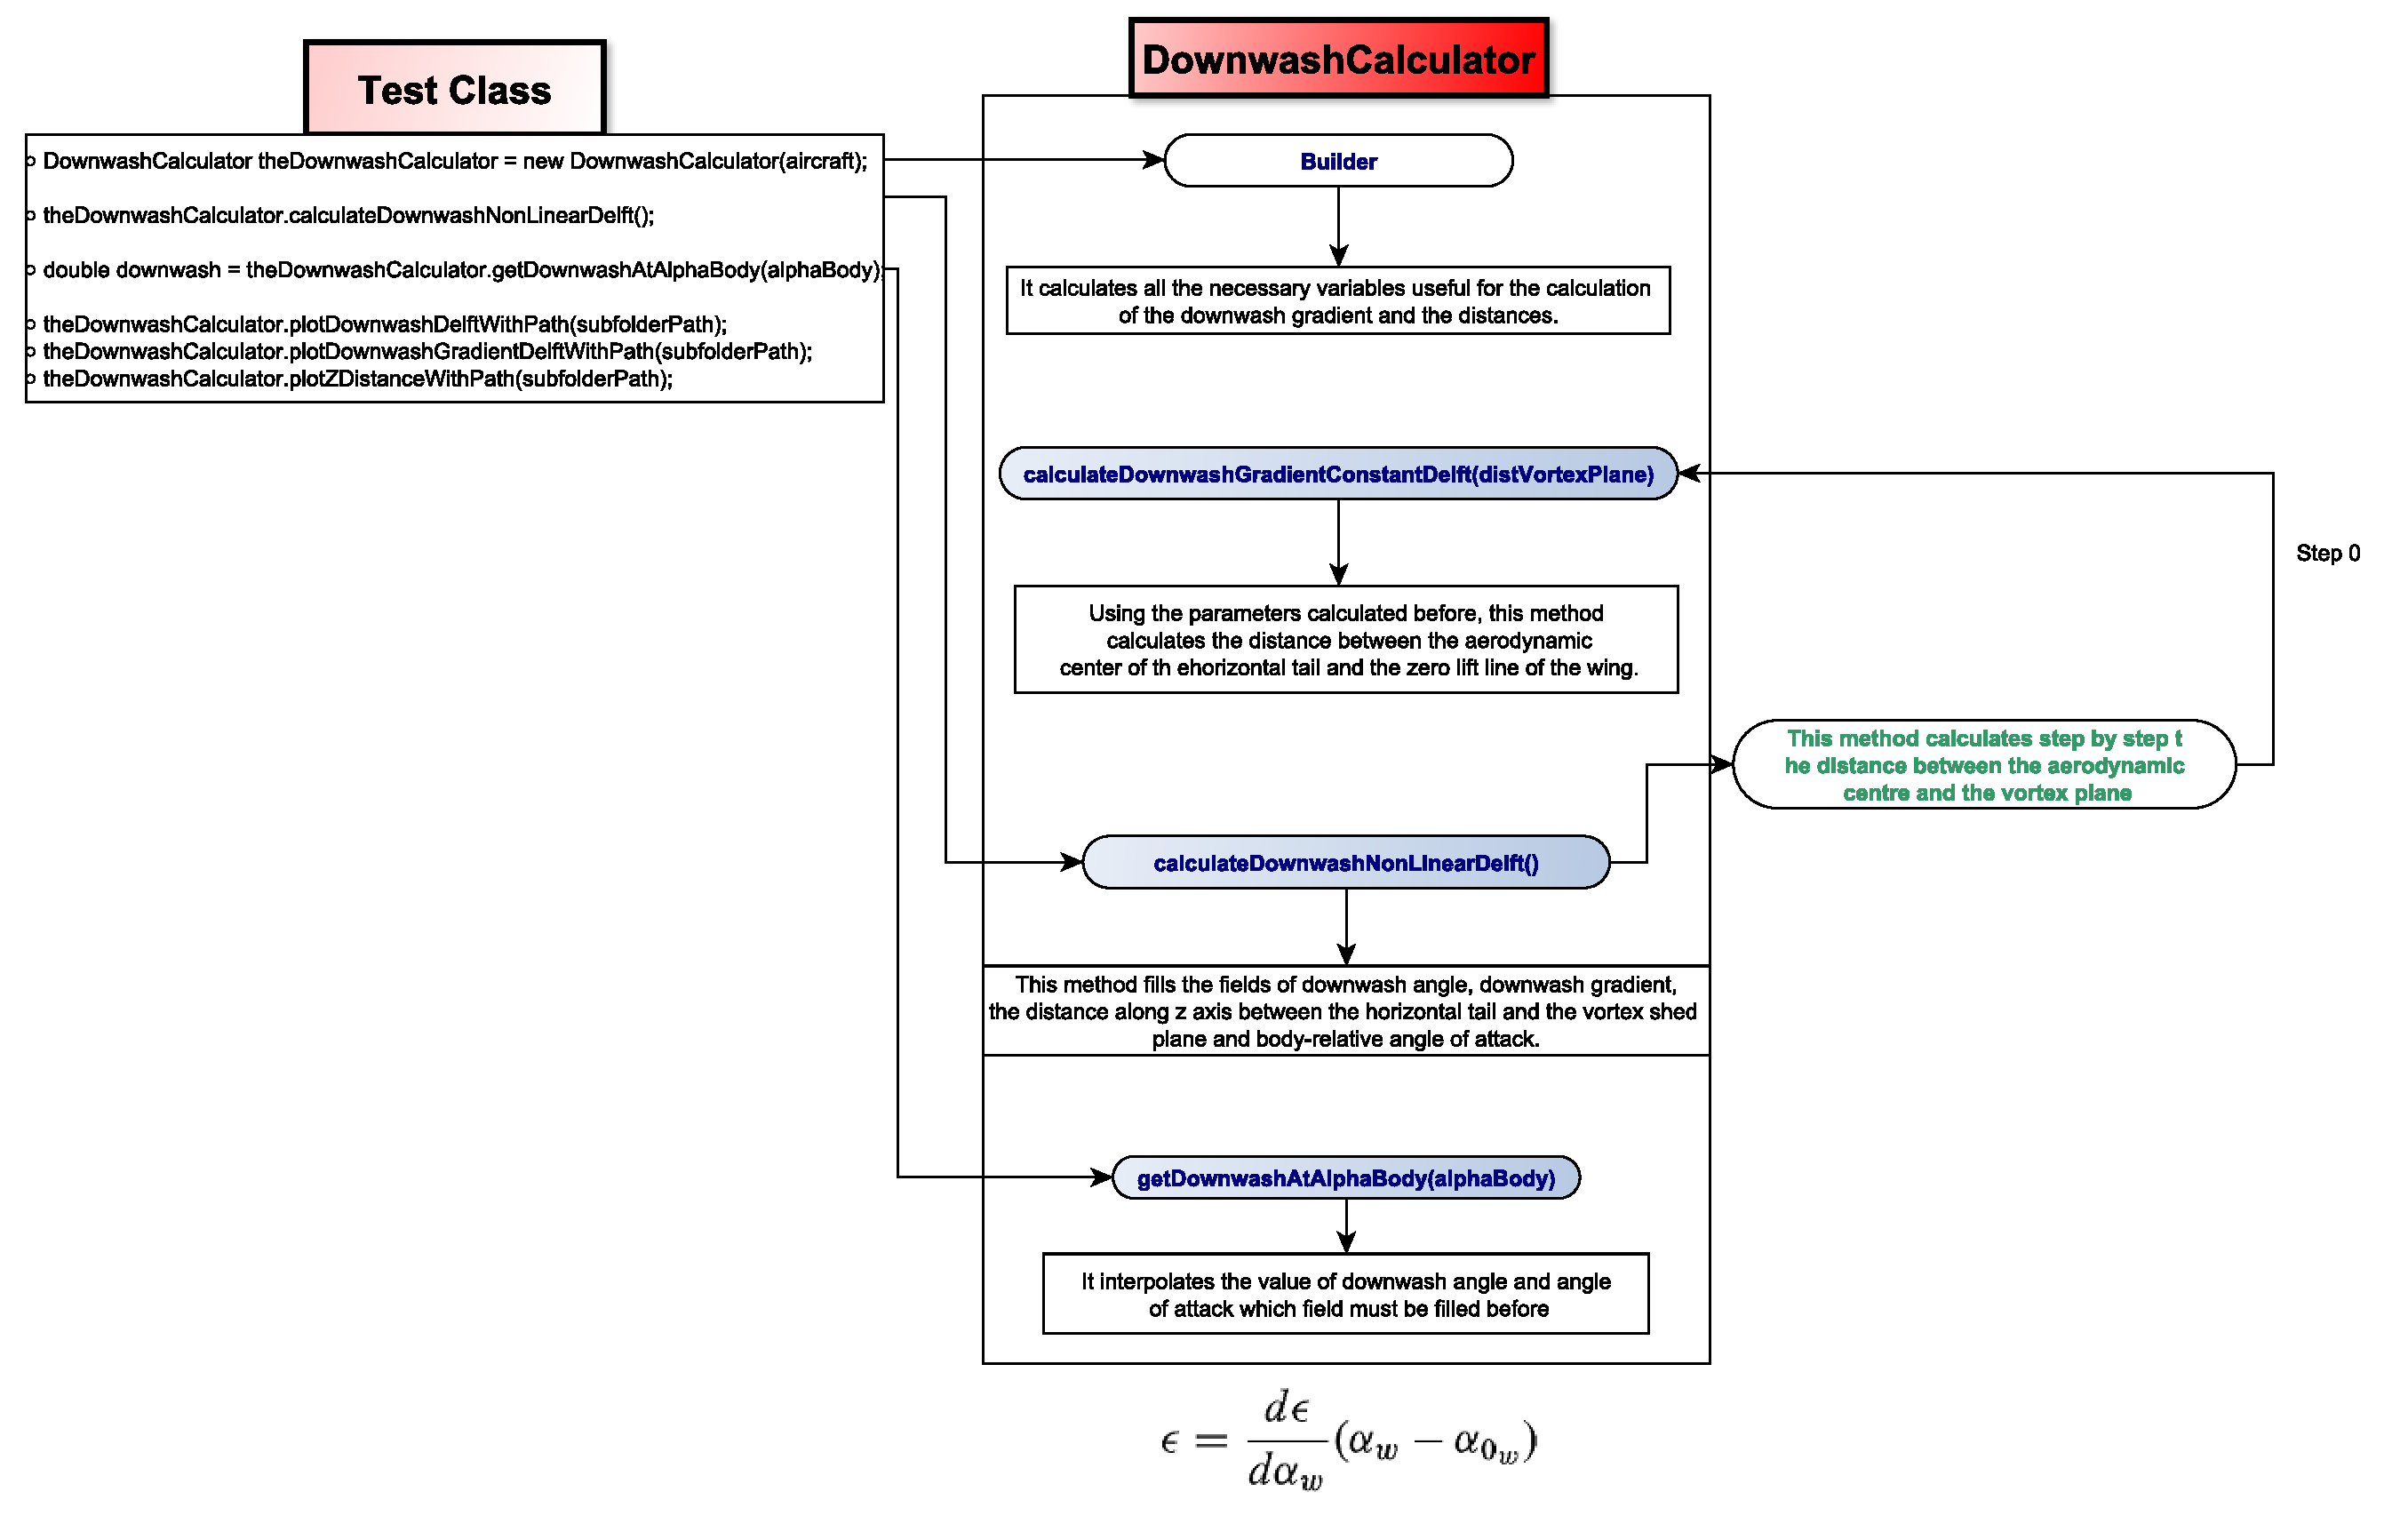
\includegraphics[height=13cm]{Immagini/nonlinear_2.pdf}} 
\caption{Flow chart of the calculation of non-linear downwash angle.}
\label{flowchartangles}
\end{figure} 


\section{Case Study}


\begin{lstlisting}[frame=rbl,caption={{\footnotesize Downwash Test Class}},label= [style=\bfseries]{Listing}]

	// -----------------------------------------------------------------------
	// INITIALIZE TEST CLASS ...
	// -----------------------------------------------------------------------

	// ------------------Downwash---------------

	System.out.println("\n-----Start of downwash calculation-----\n" );

	DownwashCalculator theDownwashCalculator = new DownwashCalculator(aircraft);

	theDownwashCalculator.calculateDownwashNonLinearDelft();

	theDownwashCalculator.plotDownwashDelftWithPath(subfolderPath);
	theDownwashCalculator.plotDownwashGradientDelftWithPath(subfolderPath);
	theDownwashCalculator.plotZDistanceWithPath(subfolderPath);
	System.out.println(" DONE PLOTTING DOWNWASH ANGLE vs ALPHA BODY");

	double downwash = theDownwashCalculator.getDownwashAtAlphaBody(alphaBody);
	Amount<Angle> downwashAmountRadiant = Amount
					.valueOf(Math.toRadians(downwash), SI.RADIAN);
			System.out.println( "At alpha " + alphaBody
					.to(NonSI.DEGREE_ANGLE)
		.getEstimatedValue() + " (deg) the downwash angle is (deg) = " + downwash );
	}
}
\end{lstlisting}

In the previous listing is reported the Test Class used in order to evaluate the variability of the downwash gradient with $\alpha_B$. First of all the test class is initialized, after an Aircraft object is defined with the related analysis classes.

%import static java.lang.Math.toRadians;
%import java.io.File;
%import javax.measure.quantity.Angle;
%import javax.measure.unit.NonSI;
%import javax.measure.unit.SI;
%import org.jscience.physics.amount.Amount;
%import aircraft.OperatingConditions;
%import aircraft.calculators.ACAnalysisManager;
%import aircraft.components.Aircraft;
%import aircraft.components.liftingSurface.LSAerodynamicsManager;
%import aircraft.components.liftingSurface.LiftingSurface;
%import configuration.MyConfiguration;
%import configuration.enumerations.DatabaseReaderEnum;
%import javafx.util.Pair;
%import writers.JPADStaticWriteUtils;
%
%public class prova {
%
%    public static void main(String[] args) {
%	System.out.println("Initializing test class...");
%	String folderPath = MyConfiguration.currentDirectoryString + File.separator
%	                 + "out" + File.separator;
%	String subfolderPath = JPADStaticWriteUtils.createNewFolder(folderPath 
%	                 + "Longitudinal_Static_Stability" + File.separator);
%
%	//------------------------------------------------------------------------
%	// Default folders creation:
%
%	MyConfiguration.initWorkingDirectoryTree();
%
%	//------------------------------------------------------------------------
%	// Operating Condition 
%
%	OperatingConditions theConditions = new OperatingConditions();
%	theConditions.set_alphaCurrent(Amount.valueOf(toRadians(2.), SI.RADIAN));
%
%	//------------------------------------------------------------------------
%	// Default Aircraft 
%	Aircraft aircraft = Aircraft.createDefaultAircraft("ATR-72");
%	System.out.println("Default aircraft: " + aircraft.get_name() + "\n");
%
%	//------------------------------------------------------------------------
%	// Wing and Tail
%	LiftingSurface theWing = aircraft.get_wing();
%	LiftingSurface horizontalTail = aircraft.get_HTail();
%
%	//------------------------------------------------------------------------
%	// Aerodynamic managers
%	ACAnalysisManager theAnalysis = new ACAnalysisManager(theConditions);
%	theAnalysis.updateGeometry(aircraft);
%	LSAerodynamicsManager theLSAnalysis = new LSAerodynamicsManager(
%			theConditions, 
%			theWing,
%			aircraft
%			); 
%
%	aircraft.get_wing().setAerodynamics(theLSAnalysis);
%
%	aircraft.get_exposedWing().updateAirfoilsGeometryExposedWing( aircraft);
%	//------------------------------------------------------------------------
%	// Set databases
%	theLSAnalysis.setDatabaseReaders(
%			new Pair(DatabaseReaderEnum.AERODYNAMIC, 
%					"Aerodynamic_Database_Ultimate.h5"),
%			new Pair(DatabaseReaderEnum.HIGHLIFT,
%			"HighLiftDatabase.h5")
%			);	
%
%	//------------------------------------------------------------------------
%	// Angle of attack
%
%	Amount<Angle> alphaBody = theConditions.get_alphaCurrent();
%
%
%	// -----------------------------------------------------------------------
%	// LIFT CHARACTERISTICS 
%	// -----------------------------------------------------------------------
%
%	LSAerodynamicsManager.CalcCLAtAlpha theCLWingCalculator = theLSAnalysis
%	                     .new CalcCLAtAlpha();
%	                     
%	double cLIsolatedWing = theCLWingCalculator
%	                      .nasaBlackwellCompleteCurve(alphaBody);



\noindent \\

Below are the charts representing the results obtained by applying the method described at ATR 72 and BOEING 747-100B.

\begin{figure}[H]
\centering
%Epsilon vs Alpha Body NEW
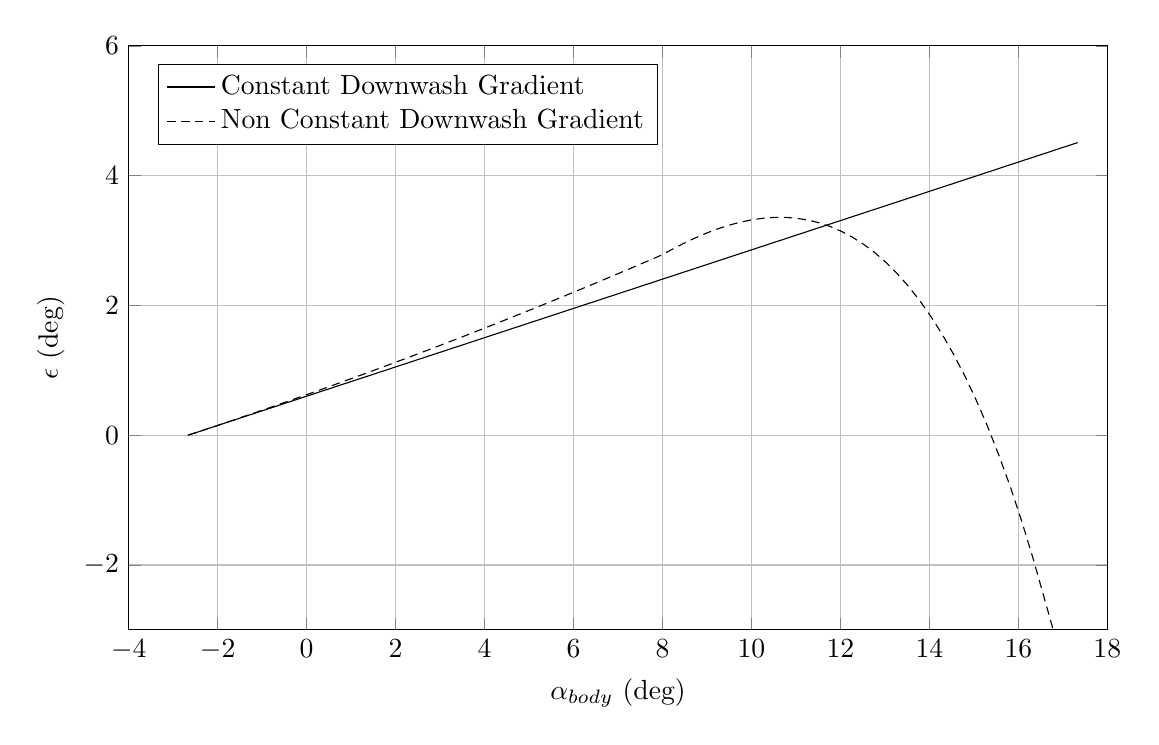
\begin{tikzpicture}

\begin{axis}[
width=14.01cm,
height=9cm,
scaled ticks=false, tick label style={/pgf/number format/fixed},
xmin=-4,
xmax=18,
xlabel={$\alpha_{body}$ (deg)},
xmajorgrids,
ymin=-3,
ymax=6,
ylabel={$\epsilon$ (deg)},
ymajorgrids,
legend style={at={(0.03,0.9)},anchor=west,draw=black,fill=white,legend cell align=left},
legend entries = {Constant Downwash Gradient\\Non Constant Downwash Gradient\\}
]

\addplot [
color=black,
solid
]
table[row sep=crcr]{
-2.6675212218928914	0.0\\
-2.4143566649308665	0.057073228053391295\\
-2.1611921079688408	0.11414645610678259\\
-1.9080275510068156	0.17121968416017389\\
-1.6548629940447903	0.22829291221356518\\
-1.401698437082765	0.2853661402669565\\
-1.1485338801207396	0.34243936832034777\\
-0.8953693231587143	0.3995125963737391\\
-0.642204766196689	0.45658582442713036\\
-0.38904020923466365	0.5136590524805217\\
-0.13587565227263831	0.570732280533913\\
0.11728890468938702	0.6278055085873042\\
0.37045346165141235	0.6848787366406955\\
0.6236180186134377	0.7419519646940869\\
0.8767825755754628	0.7990251927474782\\
1.1299471325374886	0.8560984208008695\\
1.3831116894995135	0.9131716488542607\\
1.6362762464615384	0.9702448769076519\\
1.8894408034235632	1.0273181049610431\\
2.142605360385588	1.0843913330144344\\
2.395769917347613	1.1414645610678256\\
2.648934474309638	1.1985377891212168\\
2.902099031271663	1.255611017174608\\
3.1552635882336877	1.3126842452279992\\
3.4084281451957126	1.3697574732813904\\
3.6615927021577375	1.4268307013347816\\
3.9147572591197624	1.4839039293881726\\
4.167921816081787	1.5409771574415638\\
4.421086373043812	1.598050385494955\\
4.674250930005837	1.6551236135483463\\
4.9274154869678615	1.7121968416017375\\
5.180580043929886	1.7692700696551287\\
5.433744600891911	1.8263432977085199\\
5.686909157853936	1.883416525761911\\
5.940073714815961	1.9404897538153023\\
6.193238271777986	1.9975629818686935\\
6.446402828740011	2.0546362099220845\\
6.699567385702036	2.1117094379754757\\
6.952731942664061	2.168782666028867\\
7.2058964996260855	2.225855894082258\\
7.45906105658811	2.2829291221356494\\
7.712225613550135	2.3400023501890406\\
7.96539017051216	2.397075578242432\\
8.218554727474185	2.454148806295823\\
8.47171928443621	2.511222034349214\\
8.724883841398235	2.5682952624026054\\
8.97804839836026	2.6253684904559966\\
9.231212955322285	2.682441718509388\\
9.48437751228431	2.739514946562779\\
9.737542069246334	2.7965881746161703\\
9.99070662620836	2.8536614026695615\\
10.243871183170384	2.9107346307229527\\
10.497035740132409	2.967807858776344\\
10.750200297094434	3.024881086829735\\
11.003364854056459	3.0819543148831263\\
11.256529411018484	3.1390275429365175\\
11.509693967980509	3.1961007709899087\\
11.762858524942533	3.2531739990433\\
12.016023081904558	3.310247227096691\\
12.269187638866583	3.3673204551500824\\
12.522352195828608	3.4243936832034736\\
12.775516752790633	3.481466911256865\\
13.028681309752658	3.538540139310256\\
13.281845866714683	3.5956133673636472\\
13.535010423676708	3.652686595417038\\
13.788174980638734	3.7097598234704297\\
14.041339537600761	3.7668330515238213\\
14.294504094562788	3.823906279577213\\
14.547668651524814	3.8809795076306046\\
14.800833208486841	3.9380527356839963\\
15.053997765448868	3.995125963737388\\
15.307162322410894	4.05219919179078\\
15.560326879372921	4.109272419844171\\
15.813491436334948	4.166345647897563\\
16.066655993296976	4.223418875950954\\
16.319820550259003	4.280492104004346\\
16.57298510722103	4.337565332057737\\
16.826149664183056	4.394638560111129\\
17.079314221145083	4.451711788164521\\
17.33247877810711	4.508785016217912\\
};

\addplot [
color=black,
densely dashed
]
table[row sep=crcr]{
-2.6675212218928914	0.0\\
-2.4143566649308665	0.05728316281565107\\
-2.1611921079688408	0.11498671030314704\\
-1.9080275510068156	0.17311138605812104\\
-1.6548629940447903	0.23165789459306607\\
-1.401698437082765	0.2906269010413643\\
-1.1485338801207396	0.35001903088025826\\
-0.8953693231587143	0.4098348696728695\\
-0.642204766196689	0.4700749628293539\\
-0.38904020923466365	0.530739815387257\\
-0.13587565227263831	0.5918298918111226\\
0.11728890468938702	0.6533456158113787\\
0.37045346165141235	0.7152873701825155\\
0.6236180186134377	0.7776554966605383\\
0.8767825755754628	0.8404502957996768\\
1.1299471325374886	0.9036720268682938\\
1.3831116894995135	0.9673209077639354\\
1.6362762464615384	1.0313971149474295\\
1.8894408034235632	1.0959007833959433\\
2.142605360385588	1.1608320065748656\\
2.395769917347613	1.2261908364283858\\
2.648934474309638	1.291977283388614\\
2.902099031271663	1.3581913164030675\\
3.1552635882336877	1.424832862980339\\
3.4084281451957126	1.4919018092537484\\
3.6615927021577375	1.559398000062745\\
3.9147572591197624	1.627321239051849\\
4.167921816081787	1.6956712887868595\\
4.421086373043812	1.7644478708880957\\
4.674250930005837	1.8336506661803664\\
4.9274154869678615	1.9032793148594083\\
5.180580043929886	1.9733334166744716\\
5.433744600891911	2.0438125311267616\\
5.686909157853936	2.1147161776833894\\
5.940073714815961	2.18604383600653\\
6.193238271777986	2.2577949461974116\\
6.446402828740011	2.3299689090548164\\
6.699567385702036	2.4025650863477073\\
6.952731942664061	2.4755828011016248\\
7.2058964996260855	2.5490213378984765\\
7.45906105658811	2.622879943189338\\
7.712225613550135	2.6971578256198665\\
7.96539017051216	2.771854156367948\\
8.218554727474185	2.864653388616044\\
8.47171928443621	2.9543747747747666\\
8.724883841398235	3.036760881126147\\
8.97804839836026	3.1112073833866787\\
9.231212955322285	3.1770981671898997\\
9.48437751228431	3.2338040665168535\\
9.737542069246334	3.2806809245648645\\
9.99070662620836	3.317067479180961\\
10.243871183170384	3.3422830582161596\\
10.497035740132409	3.355625068336188\\
10.750200297094434	3.3563662588253065\\
11.003364854056459	3.3437517398711845\\
11.256529411018484	3.3169957327645383\\
11.509693967980509	3.2752780274382385\\
11.762858524942533	3.217740120941675\\
12.016023081904558	3.1434810089279206\\
12.269187638866583	3.051552601243574\\
12.522352195828608	2.9409547325629624\\
12.775516752790633	2.8106297401203406\\
13.028681309752658	2.6594565835304094\\
13.281845866714683	2.4862444872616165\\
13.535010423676708	2.2897260955632612\\
13.788174980638734	2.068550144000453\\
14.041339537600761	1.8212736730538455\\
14.294504094562788	1.5463538399581198\\
14.547668651524814	1.242139428195698\\
14.800833208486841	0.9068622138132706\\
15.053997765448868	0.5386284287972798\\
15.307162322410894	0.13541066994828696\\
15.560326879372921	-0.30495925646101335\\
15.813491436334948	-0.7847958817439786\\
16.066655993296976	-1.3065631124427608\\
16.319820550259003	-1.8728735790396822\\
16.57298510722103	-2.4864827905623756\\
16.826149664183056	-3.1045405457805315\\
17.079314221145083	-3.71712306190116\\
17.33247877810711	-3.749558522643724\\
};
\end{axis}
\end{tikzpicture}%
\caption{ATR 72 Downwash angle vs $\alpha_{B}$.}
\label{fig:epsilon}
\end{figure}

\begin{figure}[H]
\centering
%Downwash gradient vs Alpha Body NEW
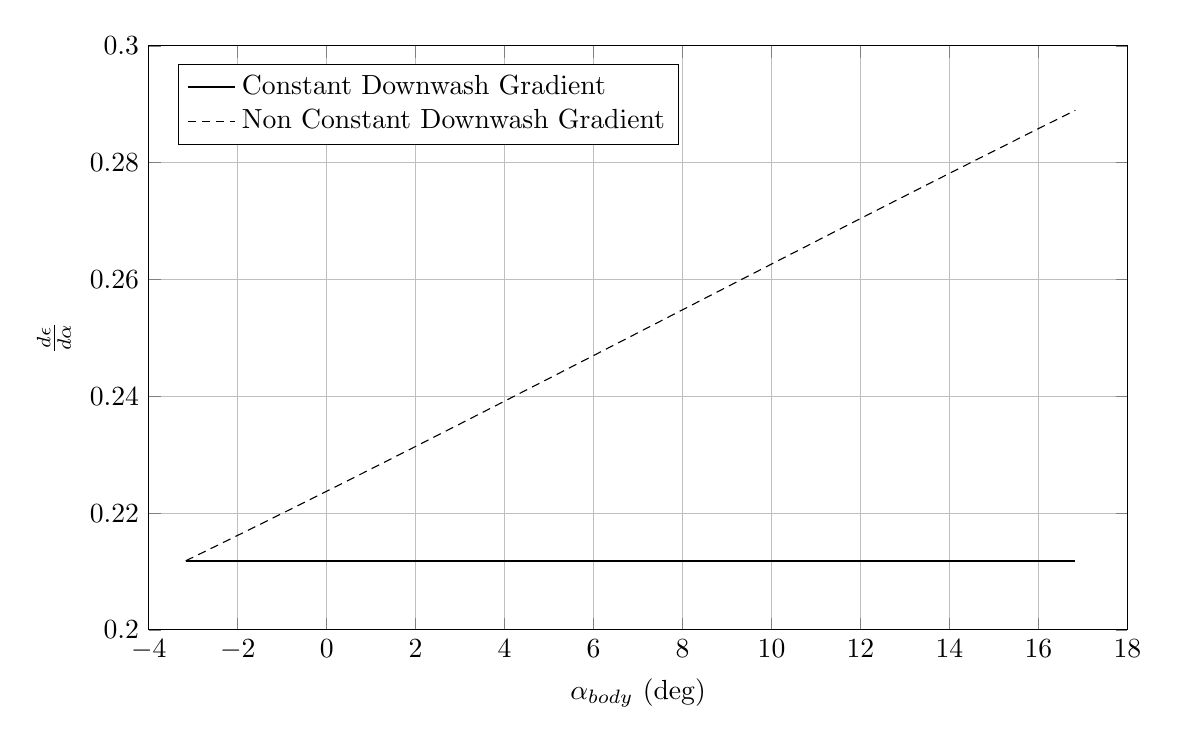
\begin{tikzpicture}

\begin{axis}[
width=14.01cm,
height=9cm,
scaled ticks=false, tick label style={/pgf/number format/fixed},
xmin=-4,
xmax=18,
xlabel={$\alpha_{body}$ (deg)},
xmajorgrids,
ymin=0.2,
ymax=0.3,
ylabel={$\frac{d \epsilon}{d \alpha}$ },
ymajorgrids,
legend style={at={(0.03,0.9)},anchor=west,draw=black,fill=white,legend cell align=left},
legend entries = {Constant Downwash Gradient\\Non Constant Downwash Gradient\\}
]

\addplot [
color=black,
thick
]
table[row sep=crcr]{
-3.169553350368967	0.21183320625402868\\
-2.9163887934069415	0.21183320625402868\\
-2.663224236444916	0.21183320625402868\\
-2.410059679482891	0.21183320625402868\\
-2.1568951225208655	0.21183320625402868\\
-1.9037305655588401	0.21183320625402868\\
-1.6505660085968148	0.21183320625402868\\
-1.3974014516347895	0.21183320625402868\\
-1.1442368946727641	0.21183320625402868\\
-0.8910723377107388	0.21183320625402868\\
-0.6379077807487135	0.21183320625402868\\
-0.3847432237866881	0.21183320625402868\\
-0.1315786668246628	0.21183320625402868\\
0.12158589013736254	0.21183320625402868\\
0.3747504470993879	0.21183320625402868\\
0.6279150040614132	0.21183320625402868\\
0.8810795610234385	0.21183320625402868\\
1.1342441179854634	0.21183320625402868\\
1.3874086749474883	0.21183320625402868\\
1.6405732319095132	0.21183320625402868\\
1.893737788871538	0.21183320625402868\\
2.146902345833563	0.21183320625402868\\
2.400066902795588	0.21183320625402868\\
2.6532314597576128	0.21183320625402868\\
2.906396016719637	0.21183320625402868\\
3.159560573681662	0.21183320625402868\\
3.412725130643687	0.21183320625402868\\
3.665889687605712	0.21183320625402868\\
3.9190542445677368	0.21183320625402868\\
4.172218801529762	0.21183320625402868\\
4.4253833584917865	0.21183320625402868\\
4.678547915453811	0.21183320625402868\\
4.931712472415836	0.21183320625402868\\
5.184877029377861	0.21183320625402868\\
5.438041586339886	0.21183320625402868\\
5.691206143301911	0.21183320625402868\\
5.944370700263936	0.21183320625402868\\
6.197535257225961	0.21183320625402868\\
6.450699814187986	0.21183320625402868\\
6.7038643711500105	0.21183320625402868\\
6.957028928112035	0.21183320625402868\\
7.21019348507406	0.21183320625402868\\
7.463358042036085	0.21183320625402868\\
7.71652259899811	0.21183320625402868\\
7.969687155960135	0.21183320625402868\\
8.22285171292216	0.21183320625402868\\
8.476016269884184	0.21183320625402868\\
8.72918082684621	0.21183320625402868\\
8.982345383808234	0.21183320625402868\\
9.23550994077026	0.21183320625402868\\
9.488674497732283	0.21183320625402868\\
9.74183905469431	0.21183320625402868\\
9.995003611656333	0.21183320625402868\\
10.24816816861836	0.21183320625402868\\
10.501332725580383	0.21183320625402868\\
10.75449728254241	0.21183320625402868\\
11.007661839504433	0.21183320625402868\\
11.26082639646646	0.21183320625402868\\
11.513990953428483	0.21183320625402868\\
11.76715551039051	0.21183320625402868\\
12.020320067352532	0.21183320625402868\\
12.273484624314559	0.21183320625402868\\
12.526649181276582	0.21183320625402868\\
12.779813738238609	0.21183320625402868\\
13.032978295200632	0.21183320625402868\\
13.286142852162659	0.21183320625402868\\
13.539307409124685	0.21183320625402868\\
13.792471966086712	0.21183320625402868\\
14.045636523048739	0.21183320625402868\\
14.298801080010765	0.21183320625402868\\
14.551965636972792	0.21183320625402868\\
14.805130193934819	0.21183320625402868\\
15.058294750896845	0.21183320625402868\\
15.311459307858872	0.21183320625402868\\
15.564623864820899	0.21183320625402868\\
15.817788421782925	0.21183320625402868\\
16.070952978744952	0.21183320625402868\\
16.32411753570698	0.21183320625402868\\
16.577282092669005	0.21183320625402868\\
16.830446649631032	0.21183320625402868\\
};

\addplot [
color=black,
densely dashed
]
table[row sep=crcr]{
-3.169553350368967	0.21183320625402868\\
-2.9163887934069415	0.21277220832857538\\
-2.663224236444916	0.21371363258684833\\
-2.410059679482891	0.21465742559910517\\
-2.1568951225208655	0.2156035334801616\\
-1.9037305655588401	0.21655190190587265\\
-1.6505660085968148	0.21750247612986656\\
-1.3974014516347895	0.21845520100051946\\
-1.1442368946727641	0.21941002097815557\\
-0.8910723377107388	0.22036688015245975\\
-0.6379077807487135	0.2213257222600863\\
-0.3847432237866881	0.22228649070245077\\
-0.1315786668246628	0.223249128563688\\
0.12158589013736254	0.22421357862876357\\
0.3747504470993879	0.2251797834017208\\
0.6279150040614132	0.22614768512405\\
0.8810795610234385	0.22711722579316368\\
1.1342441179854634	0.22808834718096105\\
1.3874086749474883	0.2290609908524691\\
1.6405732319095132	0.2300350981845411\\
1.893737788871538	0.23101061038460013\\
2.146902345833563	0.23198746850940938\\
2.400066902795588	0.23296561348385603\\
2.6532314597576128	0.23394498611973133\\
2.906396016719637	0.2349255271344935\\
3.159560573681662	0.2359071771699958\\
3.412725130643687	0.23688987681116752\\
3.665889687605712	0.23787356660463027\\
3.9190542445677368	0.2388581870772378\\
4.172218801529762	0.23984367875452164\\
4.4253833584917865	0.24082998217903084\\
4.678547915453811	0.24181703792855133\\
4.931712472415836	0.24280478663418992\\
5.184877029377861	0.24379316899831058\\
5.438041586339886	0.24478212581231037\\
5.691206143301911	0.24577159797422057\\
5.944370700263936	0.24676152650612254\\
6.197535257225961	0.24775185257136376\\
6.450699814187986	0.2487425174915651\\
6.7038643711500105	0.24973346276340555\\
6.957028928112035	0.25072463007517526\\
7.21019348507406	0.2517159613230841\\
7.463358042036085	0.2527073986273186\\
7.71652259899811	0.25369888434783416\\
7.969687155960135	0.2546903610998764\\
8.22285171292216	0.25568177176921986\\
8.476016269884184	0.2566730595271178\\
8.72918082684621	0.2576641678449536\\
8.982345383808234	0.2586550405085876\\
9.23550994077026	0.2596456216323908\\
9.488674497732283	0.26063585567295927\\
9.74183905469431	0.2616256874425042\\
9.995003611656333	0.26261506212190977\\
10.24816816861836	0.2636039252734554\\
10.501332725580383	0.2645922228531963\\
10.75449728254241	0.26557990122299874\\
11.007661839504433	0.26656690716222553\\
11.26082639646646	0.26755318787906845\\
11.513990953428483	0.268538691021525\\
11.76715551039051	0.2695233646880159\\
12.020320067352532	0.2705071574376418\\
12.273484624314559	0.2714900183000775\\
12.526649181276582	0.2724718967851024\\
12.779813738238609	0.273452742891765\\
13.032978295200632	0.2744325071171834\\
13.286142852162659	0.2754111404649787\\
13.539307409124685	0.2763885944533443\\
13.792471966086712	0.27736482112274924\\
14.045636523048739	0.2783397730432789\\
14.298801080010765	0.2793134033216125\\
14.551965636972792	0.2802856656076398\\
14.805130193934819	0.28125651410071995\\
15.058294750896845	0.2822259035555826\\
15.311459307858872	0.2831937892878761\\
15.564623864820899	0.28416012717936484\\
15.817788421782925	0.2851248736827785\\
16.070952978744952	0.28608798582631756\\
16.32411753570698	0.2870494212178181\\
16.577282092669005	0.2880091380485813\\
16.830446649631032	0.2889670950968686\\
};
\end{axis}
\end{tikzpicture}%

\caption{ATR 72 Downwash gradient vs $\alpha_{B}$.}
\label{fig:downwashgradATR}
\end{figure}

\begin{figure}[H]
\centering
\input{immagini/z.tikz}
\caption{ATR 72 Distance between AC horizontal tail and vortex plane vs $\alpha_{B}$.}
\label{fig:zATR}
\end{figure}


\begin{lstlisting}[caption={{\footnotesize Downwash estimation - Results. ATR 72}},label= [style=\bfseries]{Listing}]

-----Start of downwash calculation-----

			DONE PLOTTING DOWNWASH ANGLE vs ALPHA BODY

At alpha 1.9999999999999996 (deg) the downwash angle is (deg) = 1.2696901686304403

 
-----------angles-------------- 
Angle of attack alpha body (deg) = 2.0
Angle of incidence of horizontal tail (deg) 0.0
Downwash Angle at Alpha Body (deg) 1.2696901686304403
Angle of Attack of Horizontal Tail (deg) 0.7303098313695591
\end{lstlisting}


\noindent \\ \\
\begin{lstlisting}[caption={{\footnotesize Downwash estimation - Results. BOEING 747-100B}},label= [style=\bfseries]{Listing}]

-----Start of downwash calculation-----

			DONE PLOTTING DOWNWASH ANGLE vs ALPHA BODY

At alpha 1.9999999999999996 (deg) the downwash angle is (deg) = 2.540913931771228

 
-----------angles-------------- 
Angle of attack alpha body (deg) = 2.0
Angle of incidence of horizontal tail (deg) 0.0
Downwash Angle at Alpha Body (deg) 2.540913931771228
Angle of Attack of Horizontal Tail (deg) -0.5409139317712283
\end{lstlisting}


\begin{figure}[H]
\centering
%Epsilon vs Alpha Body NEW
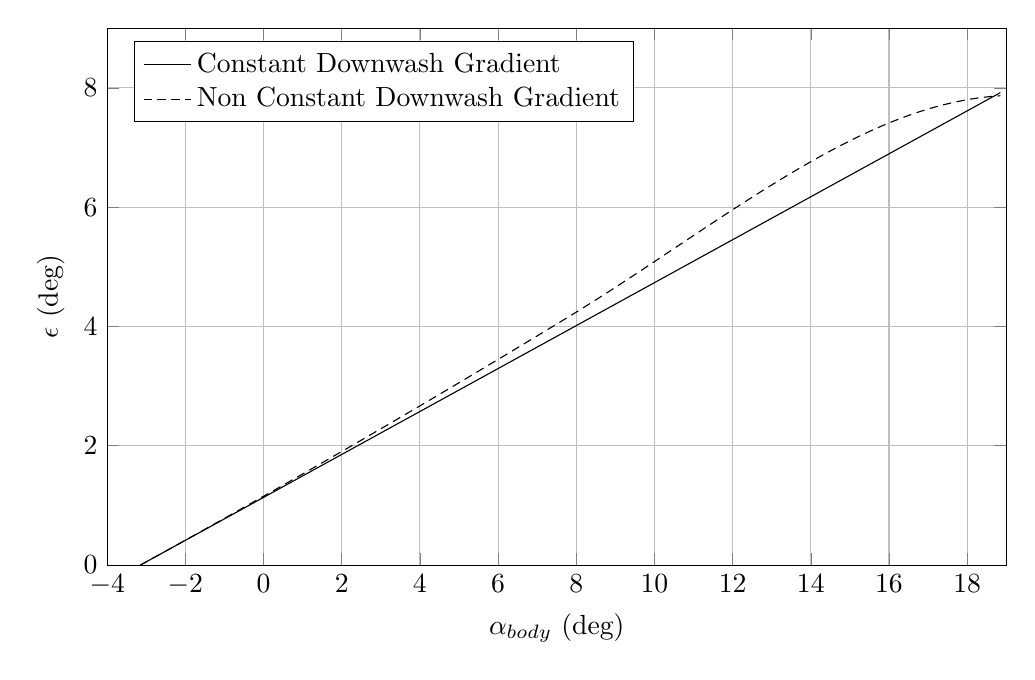
\begin{tikzpicture}

\begin{axis}[
width=13cm,
height=8.4cm,
scaled ticks=false, tick label style={/pgf/number format/fixed},
xmin=-4,
xmax=19,
xlabel={$\alpha_{body}$ (deg)},
xmajorgrids,
ymin=0,
ymax=9,
ylabel={$\epsilon$ (deg)},
ymajorgrids,
legend style={at={(0.03,0.9)},anchor=west,draw=black,fill=white,legend cell align=left},
legend entries = {Constant Downwash Gradient\\Non Constant Downwash Gradient\\}
]

\addplot [
color=black,
solid
]
table[row sep=crcr]{
-3.151545787021014	0.0\\
-2.898672223802623	0.091034202233724\\
-2.6457986605842327	0.182068404467448\\
-2.3929250973658416	0.273102606701172\\
-2.140051534147451	0.364136808934896\\
-1.8871779709290601	0.4551710111686199\\
-1.6343044077106694	0.5462052134023438\\
-1.3814308444922787	0.6372394156360678\\
-1.128557281273888	0.7282736178697917\\
-0.8756837180554973	0.8193078201035157\\
-0.6228101548371066	0.9103420223372397\\
-0.36993659161871584	1.0013762245709636\\
-0.11706302840032512	1.0924104268046875\\
0.1358105348180656	1.1834446290384115\\
0.38868409803645654	1.2744788312721353\\
0.6415576612548468	1.3655130335058594\\
0.894431224473238	1.4565472357395834\\
1.1473047876916291	1.5475814379733077\\
1.4001783509100203	1.6386156402070318\\
1.6530519141284115	1.7296498424407558\\
1.9059254773468026	1.8206840446744799\\
2.158799040565194	1.9117182469082041\\
2.411672603783585	2.002752449141928\\
2.6645461670019763	2.0937866513756522\\
2.9174197302203675	2.1848208536093763\\
3.1702932934387587	2.2758550558431003\\
3.42316685665715	2.366889258076825\\
3.676040419875541	2.457923460310549\\
3.928913983093932	2.548957662544273\\
4.181787546312323	2.639991864777997\\
4.4346611095307145	2.731026067011721\\
4.687534672749106	2.822060269245445\\
4.940408235967496	2.913094471479169\\
5.193281799185886	3.0041286737128927\\
5.4461553624042764	3.0951628759466163\\
5.699028925622667	3.1861970781803404\\
5.951902488841057	3.277231280414064\\
6.204776052059447	3.368265482647788\\
6.4576496152778375	3.4592996848815116\\
6.710523178496228	3.5503338871152357\\
6.963396741714618	3.6413680893489593\\
7.216270304933008	3.732402291582683\\
7.469143868151399	3.823436493816407\\
7.722017431369789	3.9144706960501305\\
7.974890994588179	4.005504898283855\\
8.22776455780657	4.096539100517578\\
8.48063812102496	4.187573302751302\\
8.73351168424335	4.278607504985025\\
8.98638524746174	4.36964170721875\\
9.23925881068013	4.4606759094524735\\
9.49213237389852	4.551710111686197\\
9.745005937116911	4.642744313919921\\
9.997879500335301	4.733778516153644\\
10.250753063553692	4.824812718387369\\
10.503626626772082	4.915846920621092\\
10.756500189990472	5.006881122854816\\
11.009373753208862	5.09791532508854\\
11.262247316427253	5.188949527322264\\
11.515120879645643	5.279983729555988\\
11.767994442864033	5.371017931789711\\
12.020868006082424	5.462052134023435\\
12.273741569300814	5.5530863362571585\\
12.526615132519204	5.644120538490883\\
12.779488695737594	5.735154740724607\\
13.032362258955985	5.82618894295833\\
13.285235822174375	5.917223145192054\\
13.538109385392765	6.008257347425777\\
13.790982948611155	6.099291549659502\\
14.043856511829546	6.1903257518932255\\
14.296730075047936	6.281359954126949\\
14.549603638266326	6.372394156360673\\
14.802477201484717	6.463428358594396\\
15.055350764703107	6.554462560828121\\
15.308224327921497	6.6454967630618444\\
15.561097891139887	6.736530965295568\\
15.813971454358278	6.827565167529292\\
16.066845017576668	6.918599369763015\\
16.319718580795058	7.00963357199674\\
16.57259214401345	7.100667774230463\\
16.82546570723184	7.191701976464187\\
17.07833927045023	7.282736178697911\\
17.33121283366862	7.373770380931635\\
17.58408639688701	7.464804583165359\\
17.8369599601054	7.555838785399082\\
18.08983352332379	7.646872987632806\\
18.34270708654218	7.7379071898665295\\
18.59558064976057	7.828941392100254\\
18.848454212978986	7.9199755943339865\\
};

\addplot [
color=black,
densely dashed
]
table[row sep=crcr]{
-3.151545787021014	0.0\\
-2.898672223802623	0.09126936943552681\\
-2.6457986605842327	0.18276714204907374\\
-2.3929250973658416	0.27449325154735293\\
-2.140051534147451	0.3664476235049207\\
-1.8871779709290601	0.4586301753873539\\
-1.6343044077106694	0.5510408165756214\\
-1.3814308444922787	0.6436794483916399\\
-1.128557281273888	0.7365459641250014\\
-0.8756837180554973	0.8296402490608604\\
-0.6228101548371066	0.9229621805089693\\
-0.36993659161871584	1.0165116278338469\\
-0.11706302840032512	1.110288452486069\\
0.1358105348180656	1.2042925080346667\\
0.38868409803645654	1.2985236402006177\\
0.6415576612548468	1.3929816868914182\\
0.894431224473238	1.487666478236719\\
1.1473047876916291	1.5825778366250125\\
1.4001783509100203	1.6777155767413556\\
1.6530519141284115	1.7730795056061115\\
1.9059254773468026	1.868669422614697\\
2.158799040565194	1.964485119578318\\
2.411672603783585	2.060526380765678\\
2.6645461670019763	2.156792982945643\\
2.9174197302203675	2.253284695430845\\
3.1702932934387587	2.3500012801222123\\
3.42316685665715	2.4469424915544007\\
3.676040419875541	2.5441080769421194\\
3.928913983093932	2.641497776227324\\
4.181787546312323	2.7391113221272687\\
4.4346611095307145	2.836948440183391\\
4.687534672749106	2.9350088488110186\\
4.940408235967496	3.033292259349876\\
5.193281799185886	3.131798376115375\\
5.4461553624042764	3.23052689645067\\
5.699028925622667	3.32947751077946\\
5.951902488841057	3.4286499026595196\\
6.204776052059447	3.5280437488369407\\
6.4576496152778375	3.6276587193010625\\
6.710523178496228	3.727494477340079\\
6.963396741714618	3.827550679597298\\
7.216270304933008	3.9278269761280353\\
7.469143868151399	4.028323010457128\\
7.722017431369789	4.129038419637045\\
7.974890994588179	4.230603595838436\\
8.22776455780657	4.333517998928064\\
8.48063812102496	4.437777492209091\\
8.73351168424335	4.543364271731518\\
8.98638524746174	4.650280878380527\\
9.23925881068013	4.758155669647978\\
9.49213237389852	4.866968574032422\\
9.745005937116911	4.976467207416488\\
9.997879500335301	5.086508552836874\\
10.250753063553692	5.196960541053677\\
10.503626626772082	5.3075562822041364\\
10.756500189990472	5.4182850353775365\\
11.009373753208862	5.5287550852848595\\
11.262247316427253	5.638964808743293\\
11.515120879645643	5.748623228834284\\
11.767994442864033	5.857614349294273\\
12.020868006082424	5.965769075465478\\
12.273741569300814	6.072845880409847\\
12.526615132519204	6.178798462502154\\
12.779488695737594	6.28325867162258\\
13.032362258955985	6.386221527900561\\
13.285235822174375	6.487355962681902\\
13.538109385392765	6.586573147665034\\
13.790982948611155	6.6836650882226785\\
14.043856511829546	6.778415295930189\\
14.296730075047936	6.870739711310057\\
14.549603638266326	6.960292899993278\\
14.802477201484717	7.047064909257278\\
15.055350764703107	7.130681452533785\\
15.308224327921497	7.211079715118374\\
15.561097891139887	7.288009381737997\\
15.813971454358278	7.361014624454735\\
16.066845017576668	7.4299204862068144\\
16.319718580795058	7.494436117247219\\
16.57259214401345	7.554578167491885\\
16.82546570723184	7.609968819241054\\
17.07833927045023	7.66061037362091\\
17.33121283366862	7.706256730755367\\
17.58408639688701	7.746787857438775\\
17.8369599601054	7.7820884972991085\\
18.08983352332379	7.811918116552786\\
18.34270708654218	7.836291343420321\\
18.59558064976057	7.8548491086798915\\
18.848454212978986	7.867625873510926\\
};
\end{axis}
\end{tikzpicture}%
\caption{BOEING 747-100B Downwash angle vs $\alpha_{B}$.}
\label{fig:epsilonboeing}
\end{figure}

\begin{figure}[H]
\centering
%Downwash gradient vs Alpha Body NEW
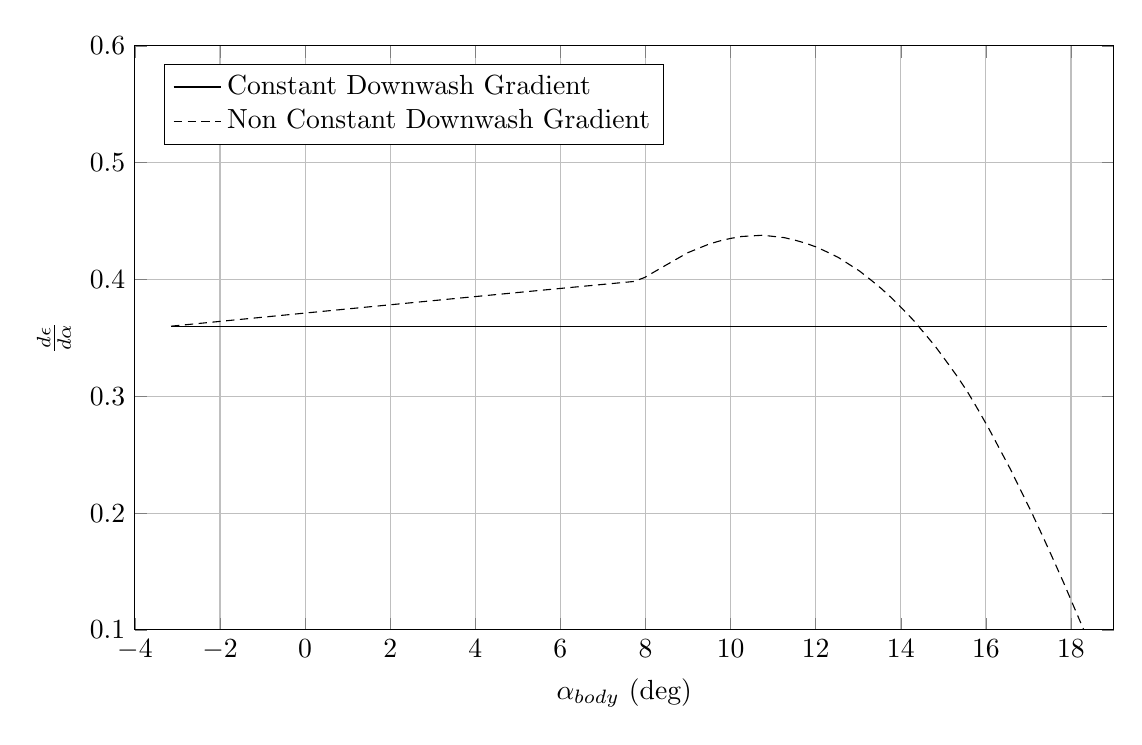
\begin{tikzpicture}

\begin{axis}[
width=14.01cm,
height=9cm,
scaled ticks=false, tick label style={/pgf/number format/fixed},
xmin=-4,
xmax=19,
xlabel={$\alpha_{body}$ (deg)},
xmajorgrids,
ymin=0.1,
ymax=0.6,
ylabel={$\frac{d \epsilon}{d \alpha}$ },
ymajorgrids,
legend style={at={(0.03,0.9)},anchor=west,draw=black,fill=white,legend cell align=left},
legend entries = {Constant Downwash Gradient\\Non Constant Downwash Gradient\\}
]

\addplot [
color=black,
solid
]
table[row sep=crcr]{
-3.151545787021014	0.35999889065154483\\
-2.898672223802623	0.35999889065154483\\
-2.6457986605842327	0.35999889065154483\\
-2.3929250973658416	0.35999889065154483\\
-2.140051534147451	0.35999889065154483\\
-1.8871779709290601	0.35999889065154483\\
-1.6343044077106694	0.35999889065154483\\
-1.3814308444922787	0.35999889065154483\\
-1.128557281273888	0.35999889065154483\\
-0.8756837180554973	0.35999889065154483\\
-0.6228101548371066	0.35999889065154483\\
-0.36993659161871584	0.35999889065154483\\
-0.11706302840032512	0.35999889065154483\\
0.1358105348180656	0.35999889065154483\\
0.38868409803645654	0.35999889065154483\\
0.6415576612548468	0.35999889065154483\\
0.894431224473238	0.35999889065154483\\
1.1473047876916291	0.35999889065154483\\
1.4001783509100203	0.35999889065154483\\
1.6530519141284115	0.35999889065154483\\
1.9059254773468026	0.35999889065154483\\
2.158799040565194	0.35999889065154483\\
2.411672603783585	0.35999889065154483\\
2.6645461670019763	0.35999889065154483\\
2.9174197302203675	0.35999889065154483\\
3.1702932934387587	0.35999889065154483\\
3.42316685665715	0.35999889065154483\\
3.676040419875541	0.35999889065154483\\
3.928913983093932	0.35999889065154483\\
4.181787546312323	0.35999889065154483\\
4.4346611095307145	0.35999889065154483\\
4.687534672749106	0.35999889065154483\\
4.940408235967496	0.35999889065154483\\
5.193281799185886	0.35999889065154483\\
5.4461553624042764	0.35999889065154483\\
5.699028925622667	0.35999889065154483\\
5.951902488841057	0.35999889065154483\\
6.204776052059447	0.35999889065154483\\
6.4576496152778375	0.35999889065154483\\
6.710523178496228	0.35999889065154483\\
6.963396741714618	0.35999889065154483\\
7.216270304933008	0.35999889065154483\\
7.469143868151399	0.35999889065154483\\
7.722017431369789	0.35999889065154483\\
7.974890994588179	0.35999889065154483\\
8.22776455780657	0.35999889065154483\\
8.48063812102496	0.35999889065154483\\
8.73351168424335	0.35999889065154483\\
8.98638524746174	0.35999889065154483\\
9.23925881068013	0.35999889065154483\\
9.49213237389852	0.35999889065154483\\
9.745005937116911	0.35999889065154483\\
9.997879500335301	0.35999889065154483\\
10.250753063553692	0.35999889065154483\\
10.503626626772082	0.35999889065154483\\
10.756500189990472	0.35999889065154483\\
11.009373753208862	0.35999889065154483\\
11.262247316427253	0.35999889065154483\\
11.515120879645643	0.35999889065154483\\
11.767994442864033	0.35999889065154483\\
12.020868006082424	0.35999889065154483\\
12.273741569300814	0.35999889065154483\\
12.526615132519204	0.35999889065154483\\
12.779488695737594	0.35999889065154483\\
13.032362258955985	0.35999889065154483\\
13.285235822174375	0.35999889065154483\\
13.538109385392765	0.35999889065154483\\
13.790982948611155	0.35999889065154483\\
14.043856511829546	0.35999889065154483\\
14.296730075047936	0.35999889065154483\\
14.549603638266326	0.35999889065154483\\
14.802477201484717	0.35999889065154483\\
15.055350764703107	0.35999889065154483\\
15.308224327921497	0.35999889065154483\\
15.561097891139887	0.35999889065154483\\
15.813971454358278	0.35999889065154483\\
16.066845017576668	0.35999889065154483\\
16.319718580795058	0.35999889065154483\\
16.57259214401345	0.35999889065154483\\
16.82546570723184	0.35999889065154483\\
17.07833927045023	0.35999889065154483\\
17.33121283366862	0.35999889065154483\\
17.58408639688701	0.35999889065154483\\
17.8369599601054	0.35999889065154483\\
18.08983352332379	0.35999889065154483\\
18.34270708654218	0.35999889065154483\\
18.59558064976057	0.35999889065154483\\
18.848454212978986	0.35999889065154483\\
};

\addplot [
color=black,
densely dashed
]
table[row sep=crcr]{
-3.151545787021014	0.35999889065154483\\
-2.898672223802623	0.36090228547549735\\
-2.6457986605842327	0.3618054496966061\\
-2.3929250973658416	0.36270835177720445\\
-2.140051534147451	0.363610959560681\\
-1.8871779709290601	0.36451324098206983\\
-1.6343044077106694	0.36541516407277647\\
-1.3814308444922787	0.36631669696525954\\
-1.128557281273888	0.3672178078976657\\
-0.8756837180554973	0.3681184652184154\\
-0.6228101548371066	0.3690186373907402\\
-0.36993659161871584	0.36991829299716783\\
-0.11706302840032512	0.3708174007439564\\
0.1358105348180656	0.37171592946547355\\
0.38868409803645654	0.3726138481285227\\
0.6415576612548468	0.37351112583661045\\
0.894431224473238	0.3744077318341603\\
1.1473047876916291	0.3753036355106647\\
1.4001783509100203	0.3761988064047803\\
1.6530519141284115	0.377093214208361\\
1.9059254773468026	0.37798682877043027\\
2.158799040565194	0.3788796201010907\\
2.411672603783585	0.3797715583753704\\
2.6645461670019763	0.3806626139370047\\
2.9174197302203675	0.3815527573021528\\
3.1702932934387587	0.3824419591630484\\
3.42316685665715	0.38333019039158317\\
3.676040419875541	0.38421742204282366\\
3.928913983093932	0.38510362535845805\\
4.181787546312323	0.38598877177017576\\
4.4346611095307145	0.38687283290297675\\
4.687534672749106	0.38775578057841004\\
4.940408235967496	0.38863758681774285\\
5.193281799185886	0.3895182238450571\\
5.4461553624042764	0.3903976640902748\\
5.699028925622667	0.3912758801921116\\
5.951902488841057	0.3921528450009571\\
6.204776052059447	0.3930285315816829\\
6.4576496152778375	0.3939029132163769\\
6.710523178496228	0.3947759634070043\\
6.963396741714618	0.3956476558779954\\
7.216270304933008	0.3965179645787581\\
7.469143868151399	0.39738686368611825\\
7.722017431369789	0.39825432760668367\\
7.974890994588179	0.40161452240225126\\
8.22776455780657	0.40694970846304435\\
8.48063812102496	0.41226853697307686\\
8.73351168424335	0.4175169641394306\\
8.98638524746174	0.42277543861163397\\
9.23925881068013	0.4265643441430519\\
9.49213237389852	0.4302738818559857\\
9.745005937116911	0.4329854286181857\\
9.997879500335301	0.4351314499556208\\
10.250753063553692	0.43675523594929644\\
10.503626626772082	0.4373236715879006\\
10.756500189990472	0.4378496349354287\\
11.009373753208862	0.4368266564645074\\
11.262247316427253	0.4357972595161692\\
11.515120879645643	0.43361726587173943\\
11.767994442864033	0.4309785935174219\\
12.020868006082424	0.42767127790597553\\
12.273741569300814	0.42340890339047826\\
12.526615132519204	0.41896344047994827\\
12.779488695737594	0.4130622184197456\\
13.032362258955985	0.4071413046855612\\
13.285235822174375	0.39991126134208654\\
13.538109385392765	0.39232996831595557\\
13.790982948611155	0.3839262116657653\\
14.043856511829546	0.37466640475778085\\
14.296730075047936	0.36507420530960166\\
14.549603638266326	0.3541160705643323\\
14.802477201484717	0.343118580224231\\
15.055350764703107	0.3306410656575163\\
15.308224327921497	0.31791516578335266\\
15.561097891139887	0.30419945569474843\\
15.813971454358278	0.28868128607786875\\
16.066845017576668	0.2724712917683876\\
16.319718580795058	0.25511120363139855\\
16.57259214401345	0.2378169534940714\\
16.82546570723184	0.21902871613870298\\
17.07833927045023	0.20024957802116145\\
17.33121283366862	0.180497298440232\\
17.58408639688701	0.16027037705428676\\
17.8369599601054	0.13958770267763762\\
18.08983352332379	0.11795389658214751\\
18.34270708654218	0.09637793418875433\\
18.59558064976057	0.07338212082453503\\
18.848454212978986	0.050522575723071124\\
};
\end{axis}
\end{tikzpicture}%

\caption{BOEING 747-100B  Downwash gradient vs $\alpha_{B}$.}
\label{fig:downwashgradboeing}
\end{figure}

\begin{figure}[H]
\centering
\input{immagini/zboeing.tikz}
\caption{BOEING 747-100B  Distance between AC horizontal tail and vortex plane vs $\alpha_{B}$.}
\label{fig:zboeing}
\end{figure}


